% Template for Cogsci submission with R Markdown

% Stuff changed from original Markdown PLOS Template
\documentclass[10pt, letterpaper]{article}

\usepackage{cogsci}
\usepackage{pslatex}
\usepackage{float}
\usepackage{caption}

% amsmath package, useful for mathematical formulas
\usepackage{amsmath}

% amssymb package, useful for mathematical symbols
\usepackage{amssymb}

% hyperref package, useful for hyperlinks
\usepackage{hyperref}

% graphicx package, useful for including eps and pdf graphics
% include graphics with the command \includegraphics
\usepackage{graphicx}

% Sweave(-like)
\usepackage{fancyvrb}
\DefineVerbatimEnvironment{Sinput}{Verbatim}{fontshape=sl}
\DefineVerbatimEnvironment{Soutput}{Verbatim}{}
\DefineVerbatimEnvironment{Scode}{Verbatim}{fontshape=sl}
\newenvironment{Schunk}{}{}
\DefineVerbatimEnvironment{Code}{Verbatim}{}
\DefineVerbatimEnvironment{CodeInput}{Verbatim}{fontshape=sl}
\DefineVerbatimEnvironment{CodeOutput}{Verbatim}{}
\newenvironment{CodeChunk}{}{}

% cite package, to clean up citations in the main text. Do not remove.
\usepackage{apacite}

% KM added 1/4/18 to allow control of blind submission


\usepackage{color}

% Use doublespacing - comment out for single spacing
%\usepackage{setspace}
%\doublespacing


% % Text layout
% \topmargin 0.0cm
% \oddsidemargin 0.5cm
% \evensidemargin 0.5cm
% \textwidth 16cm
% \textheight 21cm

\title{A Language's Unigram Entropy Distribution Predicts Self-Paced Reading
Times}


\author{{\large \bf Josef Klafka} \\ \texttt{jklafka@uchicago.edu} \\ Department of Psychology \\ University of Chicago \And {\large \bf Daniel Yurovsky} \\ \texttt{yurovsky@uchicago.edu} \\ Department of Psychology \\ University of Chicago}

\begin{document}

\maketitle

\begin{abstract}
A major line of research in the cognitive sciences has asked how
speakers and writers distribute information in the linguistic material
they produce. We provide evidence against the Uniform Information
Density hypothesis (Jaeger, 2010) which proposes that information is
transmitted at a constant rate close to channel capacity in human
communication. We instead argue that the information structure and
transmission rate in human communication varies predictably from
language to language based on phonological and syntactic features. We
draw evidence from written and spoken corpora, including corpora of
parent and child communication at various ages and large-scale online
corpora from Wikipedia in a typologically diverse collection of
languages.

\textbf{Keywords:}
Entropy; information; information theory; communication
\end{abstract}

\section{Background}\label{background}

How do people convey information in speech and text? Is there a regular
distribution to how information is conveyed across speech and text? Does
speech, with its phonological properties, different from writing, with
its semiotic properties, in how information is conveyed?

A major line of research in the current century has asked how speakers
and writers distribute information in the linguistic material they
produce. This begins with Claude Shannon in the years after World War
II. Shannon (1948) defined ``information'' as a ``reduction in
uncertainty''. Shannon followed by quantifying uncertainty in his
measure of \emph{entropy}: the amount of uncertainty on the outcome of a
random variable. Shannon proposed that the most efficient method of
sending information through a noisy channel is at a constant rate.
Genzel \& Charniak (2002) apply this principle to human communication:
if people communicate information through speech and text optimally,
then we should transmit information to one another at a constant rate.
Genzel \& Charniak created a distribution of estimates for
sentence-level entropy, each sentence taken without context, for
newspaper articles from the Penn Treebank corpus. Obtaining a roughly
monotonically increasing linear distribution, Genzel \& Charniak
proposed the \emph{Constant Entropy Rate} (CER) principle: the entropy
rate in speech and text with context should be constant as sentence
number increases. Aylett \& Turk (2004) proposed a similar principle for
the phonological level.

Jaeger (2010) extends the CER principle to all levels of human
communication: the \emph{Uniform Information Density} (UID) hypothesis.
Jaeger argues that speakers will try to distribute information more
evenly over the course of an utterance, to be as close to channel
capacity (in a Shannon sense) as possible. In particular, Jaeger singles
out the production of ``that'' at the beginning of relative clauses in
English and the use of contractions such as ``he's'' and ``you're''
versus ``he is'' and ``you are'' as instances where higher information
density in the clause elicits the production of more material by
speakers.

More recent work has stood out in contrast to the traditional UID
perspective. Zhan and Levy (2018) study Mandarin Chinese classifier use,
and find that the use of specific classifiers, versus general
classifiers, appears more often in cases where the production of the
corresponding noun is more difficult than when the production is easier,
as would be predicted by UID. The UID perspective is challenged in Yu et
al. (2016), by performing an analysis of entropy by position within
sentence in the text portion of the British National Corpus. This work
serves as the basis for ours.

\section{Methods}\label{methods}

To explore information transmission rate in speech, we used the CHILDES
TalkBank (Brown 1973; MacWhinney 2000) corpora database of spoken
adult-child conversations. We first used the Brown and Providence
English corpora from CHILDES. The Brown corpus contains individual
recordings of conversations between three children between 1.5 and
6-years-old and their families in their homes. The Providence corpus
recorded interactions between children between 1 and 3 years old and
their parents in the home. We divided each corpus by speaker into child
and non-child categories. We further divided the corpora by utterance
length, so that all sentences of length \(k\) (e.g. \(6\)) were grouped
together. Finally, within each utterance length, we computed the unigram
entropy measure for each position. We follow Yu et al. (2016) in using
the following formula for each word position X of sentences of fixed
length k from the corpus, where each \(w\) is a word occurring in
position \(X\) and \(p(w)\) is the number of times word \(w\) occurs in
position X divided by the number of total words that occur in position
\(X\) i.e.~the number of sentences of length \(k\).

\[H(X) = \sum\limits_w p(w)\log\big(p(w)\big)\]

The result of this method can be plotted for each utterance length as an
\emph{entropy curve}, which can be visually compared across utterance
length to observe the how the unigram entropy changes across absolute
positions in each of the utterances in the English CHILDES corpora. The
entropy curves capture individual variation across positions in
utterances of the same length. This allows us to directly observe and
judge the amount of variation in words that appear in an individual
position of a sentence. For speech data, which for the corpora in the
CHILDES database consists of short and often disconnected utterances
across hours of recordings, the unigram entropy measure is unaffected by
context or lack thereof in utterances by the adults and children in the
corpora. We can directly compare any two positions within utterances to
determine the amount of uncertainty, and therefore information, on
average contained by words within that position of utterances. We are
applying the same approach as in Genzel and Charniak (2003), but within
sentences instead of across sentences.

Plots for the entropy distributions are below.

\begin{CodeChunk}
\begin{figure*}[h]

{\centering 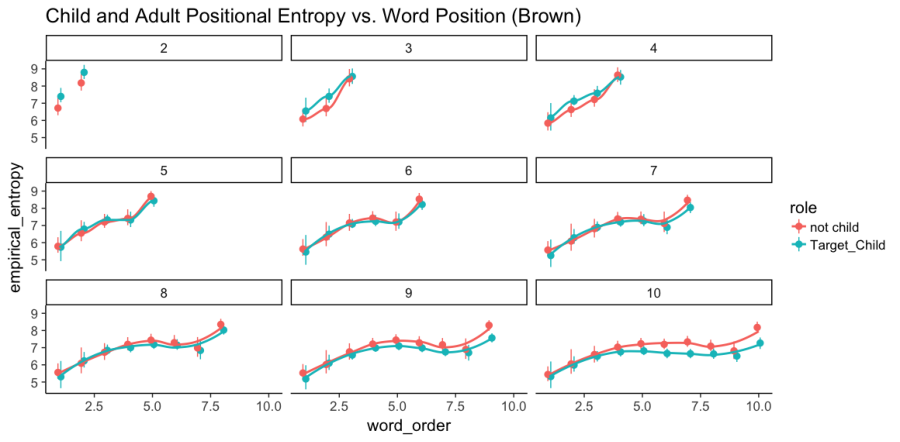
\includegraphics{figs/brown_PE-1} 

}

\caption[Brown corpus entropy]{Brown corpus entropy}\label{fig:brown_PE}
\end{figure*}
\end{CodeChunk}

\begin{CodeChunk}
\begin{figure*}[h]

{\centering 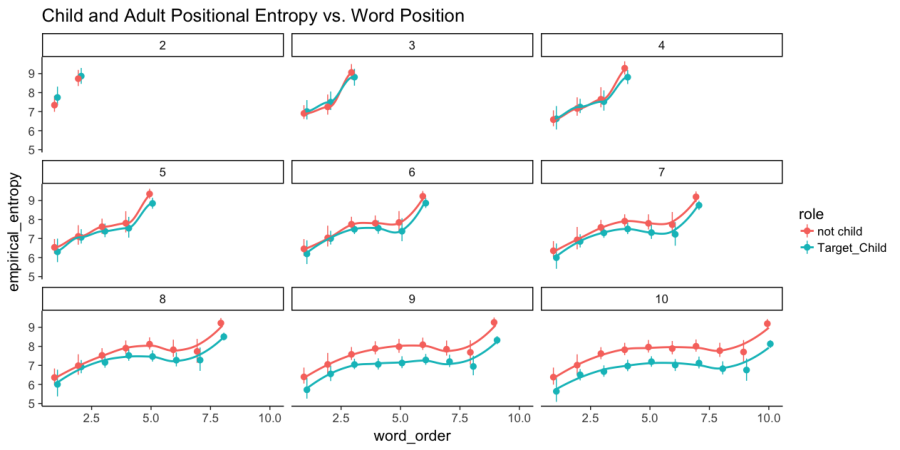
\includegraphics{figs/providence_PE-1} 

}

\caption[Providence corpus unigram entropy]{Providence corpus unigram entropy}\label{fig:providence_PE}
\end{figure*}
\end{CodeChunk}

We also ran this analysis on Spanish, German, Mandarin and Japanese
corpora from CHILDES. We used the Shiro corpus for Spanish (Shiro,
2000), which contains prompted narratives individually collected from
over a hundred Venezualan schoolchildren, half from high SES backgrounds
and half from low SES backgrounds. The German corpus we used was the
Wagner corpus of spontaneous parent-child speech in the home, collected
in single sessions for children between 1 and 14 years of age (Wagner,
1985). We used the Zhou dinner corpus for Mandarin Chinese (Li \& Zhou,
2015), which contains dinner conversations between 5 to 6-year-old
children and their parents collected in Shanghai. We used the Okayama
corpus for Japanese (Okayama, 1973), which consists of conversations
between 2 to 4-year-old children and their mothers in single sessions.

For each corpus, we accessed transcripts of the corpus provided through
the TalkBank system and computed over Roman alphabet transcriptions or
transliterations of the original transcriptions. For Mandarin, we used
pinyin transliterations of the utterances in the corpus with demarcated
word boundaries, and for Japanese we used romanji (Roman alphabet)
transliterations of words in the corpus. Japanese Hiragana, Katakana and
Kanji writing systems, and the Chinese characters used for writing
Mandarin do not normally demarcate word boundaries by spacing words
apart, and for normal Japanese and Chinese writing including spaces
between word boundaries can have a negative effect on reading times
(Sainio et al, 2007; Bai et al, 2008).

\begin{CodeChunk}
\begin{figure*}[h]

{\centering 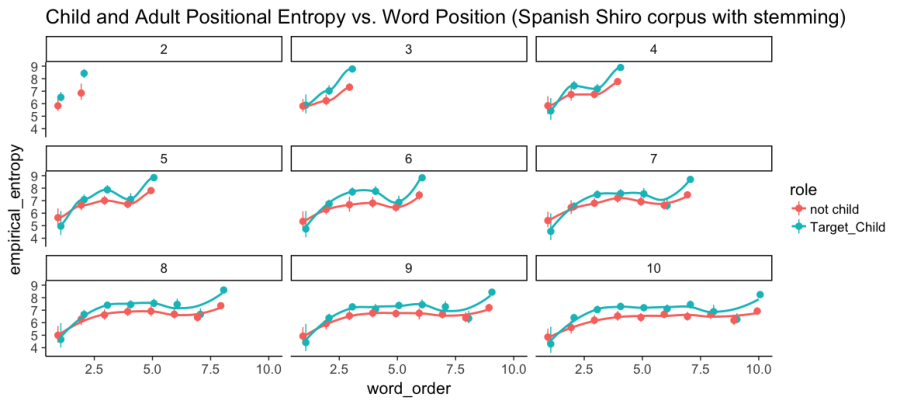
\includegraphics{figs/shiro_PE-1} 

}

\caption[Shiro corpus entropy]{Shiro corpus entropy}\label{fig:shiro_PE}
\end{figure*}
\end{CodeChunk}

\begin{CodeChunk}
\begin{figure*}[h]

{\centering 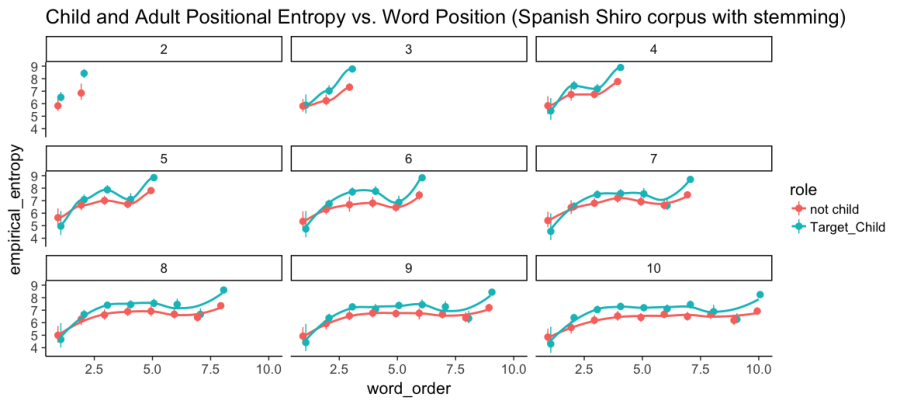
\includegraphics{figs/wagner_PE-1} 

}

\caption[Wagner corpus unigram entropy]{Wagner corpus unigram entropy}\label{fig:wagner_PE}
\end{figure*}
\end{CodeChunk}

\begin{CodeChunk}
\begin{figure*}[h]

{\centering 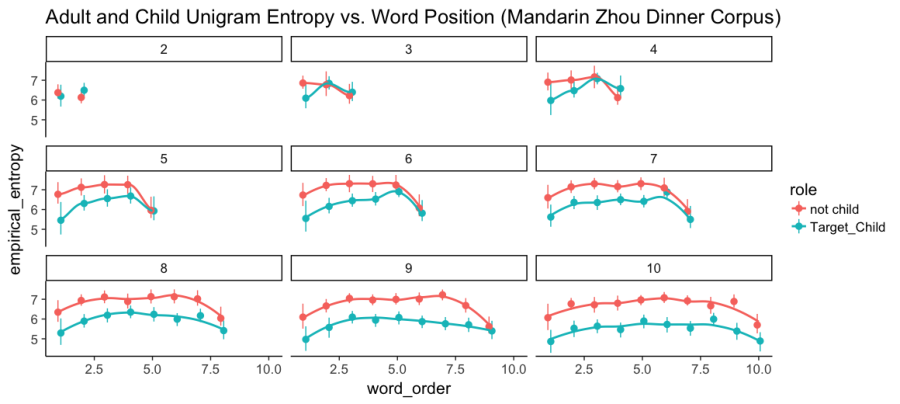
\includegraphics{figs/zhou_PE-1} 

}

\caption[Zhou Dinner corpus entropy]{Zhou Dinner corpus entropy}\label{fig:zhou_PE}
\end{figure*}
\end{CodeChunk}

\begin{CodeChunk}
\begin{figure*}[h]

{\centering 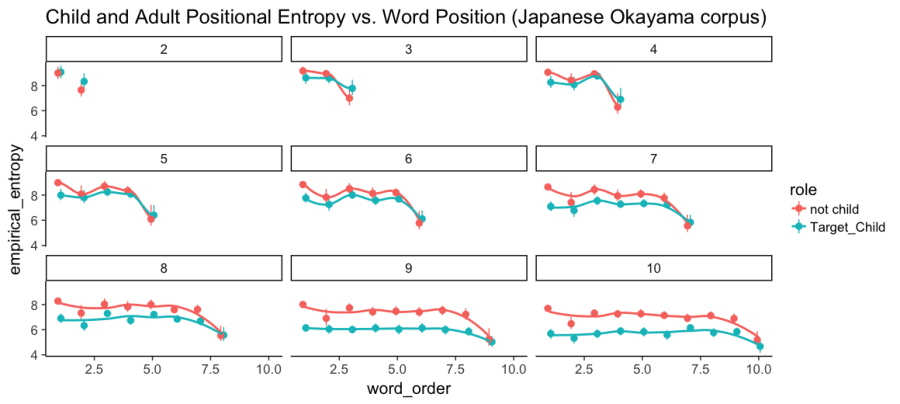
\includegraphics{figs/okayama_PE-1} 

}

\caption[Okayama corpus unigram entropy]{Okayama corpus unigram entropy}\label{fig:okayama_PE}
\end{figure*}
\end{CodeChunk}

\section{Results \& Analysis}\label{results-analysis}

The Unigram Information Density account would predict that children have
a lower channel capacity for communication and would instead communicate
with a less unigram entropy curve. The adult and child entropy curves
track one another almost identically. This not only indicates a
robustness in the unigram entropy curve across speakers, but also across
ages and addressees. We also observed a robustness across corpora for
the same languages, and a robustness across utterance lengths within the
same corpus's entropy curve. This shows that the concept of an ``entropy
curve'' for a specific language is well-founded when considering speech
data.

We found a distinct three-step distribution for English, Spanish and
German CHILDES corpora, with a slight dip in the penultimate position of
each sentence. We attribute the penultimate dip in these unigram entropy
curves to the fact that most of the utterances in the CHILDES English,
Spanish and German corpora we examined had a determiner such as ``the''
or ``a'' in the second-to-last position of utterances. The beginnings of
utterances in the English, German and Spanish CHILDES data were usually
pronouns or grammatical subjects, while the final words were grammatical
objects and had a great deal of variation in the exact word that
appeared in the utterance-final position. The final position of
utterances in child-directed speech is known to be important, dating
back to Aslin (1993). The Mandarin and Japanese data, by comparison,
have noticeably lower positional entropy values in utterance-final
positions than in utterance-penultimate positions. The Japanese entropy
curve begins high and then drops, unlike all of the other entropy
curves.

\begin{CodeChunk}
\begin{figure*}[h]

{\centering 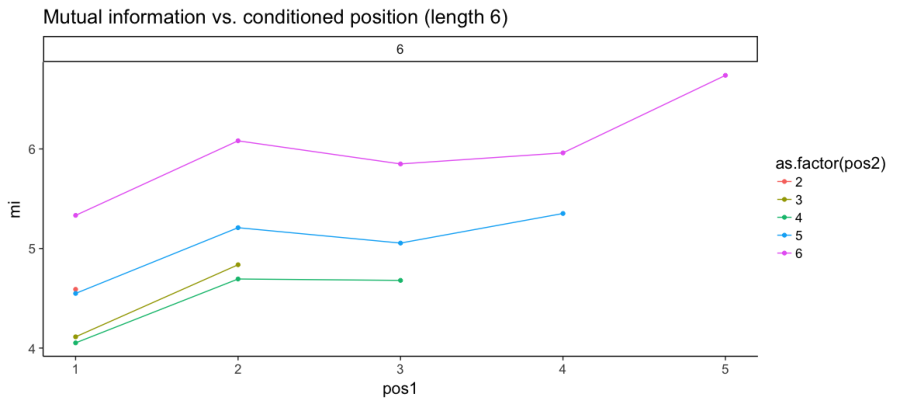
\includegraphics{figs/MI_wagner-1} 

}

\caption[Mutual Information measures on utterances of length 6 in the Wagner corpus]{Mutual Information measures on utterances of length 6 in the Wagner corpus}\label{fig:MI_wagner}
\end{figure*}
\end{CodeChunk}

\begin{CodeChunk}
\begin{figure*}[h]

{\centering 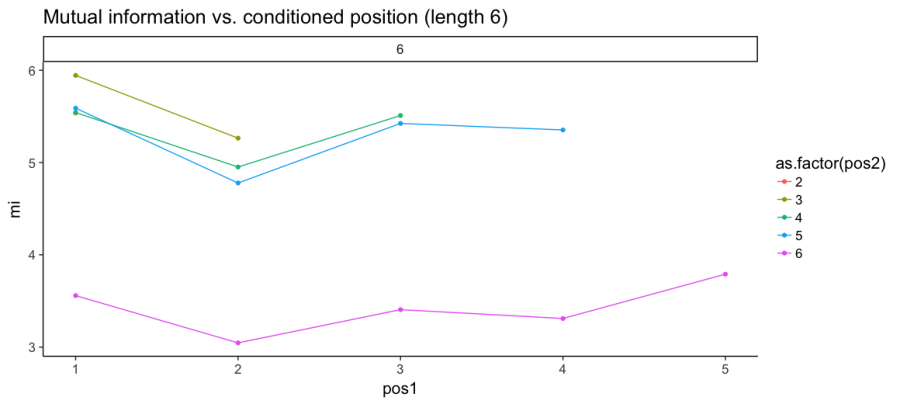
\includegraphics{figs/MI_okayama-1} 

}

\caption[Mutual Information measures on utterances of length 6 in the Okayama corpus]{Mutual Information measures on utterances of length 6 in the Okayama corpus}\label{fig:MI_okayama}
\end{figure*}
\end{CodeChunk}

The mutual information statistic is a symmetric measure of the
information gained about one random variable by learning about another,
a bigram measure and indicator of the effect than the context of a word
can have on its unigram entropy value. As seen in the images below, the
final word in utterances of length \(6\) in German has a significant
mutual information value with all other words in the utterance on
average. This means that the words appearing in positions \(1\) through
\(5\) all play a role in determining the word that appears in position
\(6\) and vice versa. By contrast, the words that appear in positions
\(1\) through \(4\) have little influence in determining the word that
appears in position \(5\), the penultimate word that is often a
determiner or function word, and instead the final word has the greatest
influence in determining the penultimate word. For Japanese, the final
word in an utterance has little to no influence on determining the rest
of the words and vice versa, whereas the other words all play in role in
determining what will go in each other's positions.

\section{Large-scale text data}\label{large-scale-text-data}

We also wanted to apply this analysis to large-scale text data, to
compare with the parent-child speech data results from using CHILDES.
Using Giuseppe Attardi's Wikiextractor tool
\footnote{https://github.com/attardi/wikiextractor}, we extracted the
text corpora for \(165\) languages from Wikipedia by downloading a
stored collection of Wikipedia entries in each langauge and randomly
selecting several thousand articles from each Wikipedia language. Each
language corpus was cleaned and limited to sentences between \(6\) and
\(50\) words. Similar to the data from CHILDES, we divided each corpus
by sentence length, and then computed the unigram entropy measure on
each word position within each sentence length.

To classify the unigram entropy curves of the different distributions,
we computed three slope treatments of each curve. In the \emph{absolute}
treatment, with sentence length denoted as \(n\), we computed the slope
between positions \(1\) and \(2\), positions \(2\) and \(3\), positions
\(3\) and \(n-2\), positions \(n-2\) and \(n-1\) and positions \(n-1\)
and \(n\). For the short utterances appearing the CHILDES speech corpora
we examined, these appeared to be important junctions in the
distributions, with a seeming plateau in the middle of the unigram
entropy curve for each of the language corpora we examined in CHILDES.

However, because the portion of sentences of length greater than \(10\)
in the Wikipedia corpora were significantly larger than the CHILDES
corpora, then we also computed relative slope treatments. In the
\emph{relative 5} treatment, we computed the slopes between \(0\%\) and
\(20\%\), \(20\%\) and \(40\%\), \(40\%\) and \(60\%\), \(60\%\) and
\(80\%\) and \(80\%\) and \(100\%\) of the relative word positions in
each sentence. When one of these percentages was not a whole number,
then the closest whole number position was used instead for slope
calculation. In the \emph{relative 10} treatment, we computed the slopes
between every \(10\%\) of the relative word positions in each sentence.
Each comparative slope within each treatment was averaged together
between different sentence lengths, for example in the \emph{relative 5}
treatment then all of the \(0\%\) to \(20\%\) slopes were averaged
together. This created three treatments for the entropy curve for each
langauge in the Wikipedia database.

For the German and Japanese entropy curves, we observed the same shape
for the text Wikipedia corpora entropy curves and the speech CHILDES
corpora entropy curves, supporting the argument for robustness across
text and speech.

\subsection{Clustering}\label{clustering}

In the \emph{absolute} and \emph{relative 5} treatments, each language
is cast as a point in \(5\)-dimensional space. In the \emph{relative 10}
treatment, each language is cast as a point in \(10\)-dimensional space.
This allows for direct comparison using cosine similarity and moreover
for unsupervised clustering analysis to compare the results of the
Wikipedia entropy analysis to known typological features within the
langauges in the Wikipedia dataset. Using the R hclust package, we
performed a hierarchical clustering of the Wikipedia slope data within
each treatment. A subset of the results at a glance for the
\emph{absolute} treatment are below.

\begin{CodeChunk}
\begin{figure*}[h]

{\centering 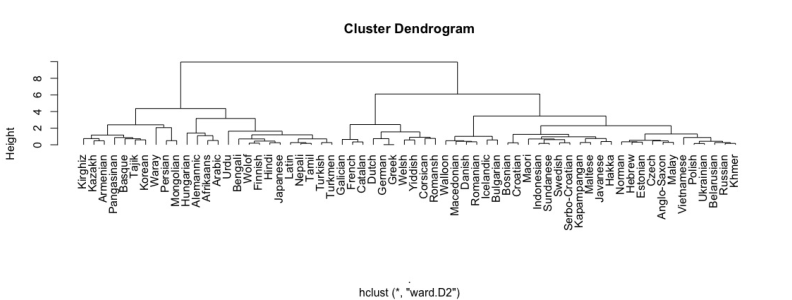
\includegraphics{figs/absolute_clusters-1} 

}

\caption[Absolute clustering of Wikipedia corpora]{Absolute clustering of Wikipedia corpora}\label{fig:absolute_clusters}
\end{figure*}
\end{CodeChunk}

\subsection{Language Features}\label{language-features}

To determine which phonological, morphological and syntactic features
affected the embedding of a language in the Wikipedia dataset, we looked
at the list of \(144\) linguistic features in World Atlas of Language
Structures (Dryer \& Haspelmath, 2013). We limited the languages in the
WALS database to only those in our Wikipedia dataset and performed
missing-value imputation to obtain the features not coded in WALS for
the languages from Wikipedia. We then performed k-modes clustering and
compared the results with the hierarchical clustering from Wikipedia.
{[}Still working on this{]}

We also checked the effects of individual features on the embeddings of
languages in the different treatments. {[}Still working on this{]}

\section{Conclusions}\label{conclusions}

In this paper we have explored the differences in rate of information
transmission among spoken child-adult conversational corpora in several
languages and text corpora pulled from Wikipedia for well over a hundred
other corpora. We have seen that the entropy curve, a representation of
information at each position of an utterance without regard to context,
varies from language to language and is predicted by a subset of
syntactic, phonological and morphological features in a language. We
have provided evidence against the Uniform Information Density
hypothesis and provided an alternate explanation for the rate at which
information is encoded and transmitted in human communication, namely
one that is robust across corpora, language dependent and arises from
the features of the language.

A large volume of research has indicated the effects of surprisal on
fixation duration during eye-tracking studies: higher surprisal of a
word corresponds to higher fixation duration. The \emph{wrap-up effect}
is a popular hypothesis within the eye-tracking community. The
hypothesis states that, in written text, sentence-final words are
processed more slowly on average then sentence-medial or
sentence-initial words, due to readers integrating information from the
entire sentence in order to form a final, coherent thought expressed by
the sentence, among other reasons. The wrap-up effect is drawn from
evidence in English, German and Dutch, all of which are languages with a
large final increase in their entropy curve from our study. We aim to
see in the future if as a consquence of our work in this paper, the
wrap-up effect falls out from the final jump in the entropy curves in
some languages.

\setlength{\parindent}{-0.1in} \setlength{\leftskip}{0.125in} \noindent

\bibliographystyle{apacite}


\end{document}
